\documentclass[11,]{article}
\usepackage{lmodern}
\usepackage{amssymb,amsmath}
\usepackage{ifxetex,ifluatex}
\usepackage{fixltx2e} % provides \textsubscript
\ifnum 0\ifxetex 1\fi\ifluatex 1\fi=0 % if pdftex
  \usepackage[T1]{fontenc}
  \usepackage[utf8]{inputenc}
\else % if luatex or xelatex
  \ifxetex
    \usepackage{mathspec}
  \else
    \usepackage{fontspec}
  \fi
  \defaultfontfeatures{Ligatures=TeX,Scale=MatchLowercase}
\fi
% use upquote if available, for straight quotes in verbatim environments
\IfFileExists{upquote.sty}{\usepackage{upquote}}{}
% use microtype if available
\IfFileExists{microtype.sty}{%
\usepackage[]{microtype}
\UseMicrotypeSet[protrusion]{basicmath} % disable protrusion for tt fonts
}{}
\PassOptionsToPackage{hyphens}{url} % url is loaded by hyperref
\usepackage[unicode=true]{hyperref}
\PassOptionsToPackage{usenames,dvipsnames}{color} % color is loaded by hyperref
\hypersetup{
            colorlinks=true,
            linkcolor=Maroon,
            citecolor=Blue,
            urlcolor=blue,
            breaklinks=true}
\urlstyle{same}  % don't use monospace font for urls
\usepackage[margin=1in]{geometry}
\usepackage{longtable,booktabs}
% Fix footnotes in tables (requires footnote package)
\IfFileExists{footnote.sty}{\usepackage{footnote}\makesavenoteenv{long table}}{}
\usepackage{graphicx,grffile}
\makeatletter
\def\maxwidth{\ifdim\Gin@nat@width>\linewidth\linewidth\else\Gin@nat@width\fi}
\def\maxheight{\ifdim\Gin@nat@height>\textheight\textheight\else\Gin@nat@height\fi}
\makeatother
% Scale images if necessary, so that they will not overflow the page
% margins by default, and it is still possible to overwrite the defaults
% using explicit options in \includegraphics[width, height, ...]{}
\setkeys{Gin}{width=\maxwidth,height=\maxheight,keepaspectratio}
\IfFileExists{parskip.sty}{%
\usepackage{parskip}
}{% else
\setlength{\parindent}{0pt}
\setlength{\parskip}{6pt plus 2pt minus 1pt}
}
\setlength{\emergencystretch}{3em}  % prevent overfull lines
\providecommand{\tightlist}{%
  \setlength{\itemsep}{0pt}\setlength{\parskip}{0pt}}
\setcounter{secnumdepth}{5}
% Redefines (sub)paragraphs to behave more like sections
\ifx\paragraph\undefined\else
\let\oldparagraph\paragraph
\renewcommand{\paragraph}[1]{\oldparagraph{#1}\mbox{}}
\fi
\ifx\subparagraph\undefined\else
\let\oldsubparagraph\subparagraph
\renewcommand{\subparagraph}[1]{\oldsubparagraph{#1}\mbox{}}
\fi

% set default figure placement to htbp
\makeatletter
\def\fps@figure{htbp}
\makeatother

%%% .rmd + .sty setup borrowed from: https://github.com/oganm/ThesisProposal

% Must load tex packages here (import.sty run in preamble, title.sty run after)
\usepackage{setspace} % for title page spacing
\usepackage{hyperref} % for all sorts of linking

\author{}
\date{\vspace{-2.5em}}

\usepackage{amsthm}
\newtheorem{theorem}{Theorem}[section]
\newtheorem{lemma}{Lemma}[section]
\theoremstyle{definition}
\newtheorem{definition}{Definition}[section]
\newtheorem{corollary}{Corollary}[section]
\newtheorem{proposition}{Proposition}[section]
\theoremstyle{definition}
\newtheorem{example}{Example}[section]
\theoremstyle{definition}
\newtheorem{exercise}{Exercise}[section]
\theoremstyle{remark}
\newtheorem*{remark}{Remark}
\newtheorem*{solution}{Solution}
\begin{document}

%%% .rmd + .sty setup borrowed from: https://github.com/oganm/ThesisProposal

\onehalfspacing
\pagenumbering{gobble}

%\begin{titlepage}
\begin{center}
\LARGE{\textbf{Dynamic visualization of high-dimensional data via
low-dimension projections and sectioning across 2D and 3D display devices}}\\
\vspace*{2\baselineskip}
\Large{\textbf{Mid canidature review}}\\
\normalsize{Monash University, Faculty of Information Technology}\\
\vspace*{2\baselineskip}
\Large{Nicholas Spyrison}\\ %, B.Sc
\vspace*{3\baselineskip}
\Large{\textbf{Thesis Supervisors}}\\
Prof. Kimbal Marriott\\
Prof. Dianne Cook\\
\vspace*{2\baselineskip}
\Large{\textbf{Committee Members}}\\
Dr. Maxime Cordiel\\
Dr. Shirui Pan\\
\vspace*{1\baselineskip}
\Large{\textbf{Chair}}\\
Assoc. Prof. Bernhard Jenny\\
\vspace*{1\baselineskip}
\Large{\textbf{Presention Date}}\\
DD Feburuary, 2020
\end{center}
% \end{titlepage}

\doublespacing

\hypersetup{linkcolor = blue}
\newpage
\pagenumbering{roman}
\tableofcontents
\addcontentsline{toc}{section}{\contentsname}

\newpage

%% list of figures have to be added manually to table of contents
% \listoffigures 
% 
% \newpage
% \listoftables

\doublespacing

\newpage
\pagenumbering{arabic}
\hypersetup{linkcolor = blue}

{
\hypersetup{linkcolor=black}
\setcounter{tocdepth}{2}
\tableofcontents
}
\section{Introduction}\label{sec:intro}

\subsection{Motivation}\label{motivation}

The term exploratory data analysis was coined by J. W. Tukey (1977), who
leaves it as an intentionally broad term that encompasses the initial
summarization and visualization of a data set. This is a critical first
step of checking for realistic values and validating model assumptions.
It may be tempting to review a series of summary statistics to check
model assumptions. However, there are known datasets where the same
summary statistics miss glaringly obvious visual patterns (Anscombe
1973; Matejka and Fitzmaurice 2017). It is strikingly simple to look at
the wrong, or incomplete set of statistics needed to validate
assumptions. Data visualization is fast, versatile, and robust relative
to the alternative of numeric statistical summarization. Data
visualization does and must remain a primary component of data analysis
and model validation.

Consider tabular data containing many attributes (variables).
Visualization of this ubiquitous type of dataset is key to its
understanding and exploration. Visualization of spaces in more than 3
dimensions quickly becomes problematic. We will discuss the use of
linear projections to mitigate this obstacle. The motivation for this
research is two-fold: expand the dimensionality support and improve the
understanding from such visualizations.

\subsubsection{Current state of the
field}\label{current-state-of-the-field}

Consider plotting 2 variables as an XY scatterplot. To add a 3rd
variable append the z-axis orthogonal (right angle to) the XY plane.
Adding a 4th dimension is not so easily solved. To resolve this we will
use scatterplot matrices to introduce axes and bases. Then we generalize
to linear projections before discussing principal component analysis and
introducing tours.

Scatterplot matrices (Chambers et al. 1983) plot every combination of
variable pairs and views them in a matrix. This is a good method to
check variable ranges and extreme values but is not the ideal
visualization. Consider a bar stool as in figure \ref{fig:basisExample}.
Given 3 still-frames of the variable-pair (that is, a square-on view
from each dimension) does not necessarily convey the full information of
the data. For instance, a three-quarter perspective helps relate the
square on images and are ubiquitous in assembly and machining
instructions. This perspective relates information contained in the view
of sides. Mathematically, we describe the angle of view as a
\texttt{basis}. Bases (plural of basis) are depicted as unit axes, they
point in the direction each dimension is oriented. The axes for the
three-quarter perspective differ from the square-on views in that the
directions are a combination of 2 and 3 variables respectively, rather
than one variable mapped fully to the horizontal or vertical.

Building on pairs of variables, an arbitrary \texttt{p} variables can be
projected down to 2 dimensions. This seems unintuitive at first, but we
have already discussed some trivial cases with scatterplot matrices.
Consider figure \ref{fig:basisExample} again. The first 3 cases plot
pairs variables, while the third direction extends directly beyond the
XY plane. These are trivial projections of 3- down to 2- dimensions,
where the 3rd variable has no contribution with a row of zeros in the
basis. The three-quarter perspective is more interesting as more than
one variable contributes to each direction. The resulting plot is said
to be a \emph{linear projection} when the basis is produced with an
affine transformation, that is, any transformation in which all parallel
lines remain parallel. One crucial aspect of linear projections is that
they are interoperable back to the original attributes; any observation
identified in any linear projection can be mapped back to its variable
values. Recently, some non-linear projection techniques such as
self-organizing maps (Kohonen 1990) and t-distributed stochastic
neighbor embedding (Maaten and Hinton 2008) have received a substantial
following. However, due to their non-linear transformation observations
cannot be mapped back to the original attribute-space and interpretation
becomes opaque. For this reason, non-linear transformations are
precluded from the exploration of data- or parameter-spaces.

Principal component analysis (PCA; Pearson 1901) is one common way of
identifying projections to consider. In PCA the new components are
formed from a linear combination of the original attributes. The new
components must be orthogonal to all previous components and ordered by
descending variation explained. A pair of these new components are then
viewed as an XY scatterplot. This has the added benefit of viewing the
most variation in as few dimensions as possible. The scree plot/test
(Cattell 1966) can be used on the components to quickly zero in on a
space that has the intrinsic dimensionality of the data. This is a
common data processing step once the number of attributes becomes
sizable (larger than 10 or so).

\subsection{From discrete to
continuous}\label{from-discrete-to-continuous}

The above methods have suggested a \emph{discrete} number of linear
projections to look at. At the same time, the stool example illustrates
that looking at intermediate views improves understanding. A
\emph{continuous} animation of the object being rotated would improve
this understanding even further. This is analogous to the idea of a data
visualization \emph{tour}(Asimov 1985; Buja and Asimov 1986). A tour
produces a relatively high number of linear projections and views them
in quick succession, typically as an animation. When the bases have a
relatively small change in the contributions the projections are much
closer. Single points and features can be tracked and follow from
projection to projection allowing for a better understanding of the
local structure.

One key feature of tours is the selection of the path animated. Asimov
originally purposed a \emph{grand} tour. In the grand tour, several
target planes are identified somewhat close to the starting basis. Many
interim planes are found between target planes via geodesic
interpolation. Figure \ref{fig:grandFrames} illustrates a simplification
of this process. A \emph{little} tour (Wickham et al. 2011) starts on a
basis with only 2 variables contributing and trades the contribution one
variable for another single variable. This effectively animates between
the planes displayed in a scatterplot matrix. A \emph{local} tour
explores a dense area of the possible projections around the initiated
basis. It walks a short distance away before returning to the starting
basis and selecting a new random frame very nearby.

\begin{figure}

{\centering 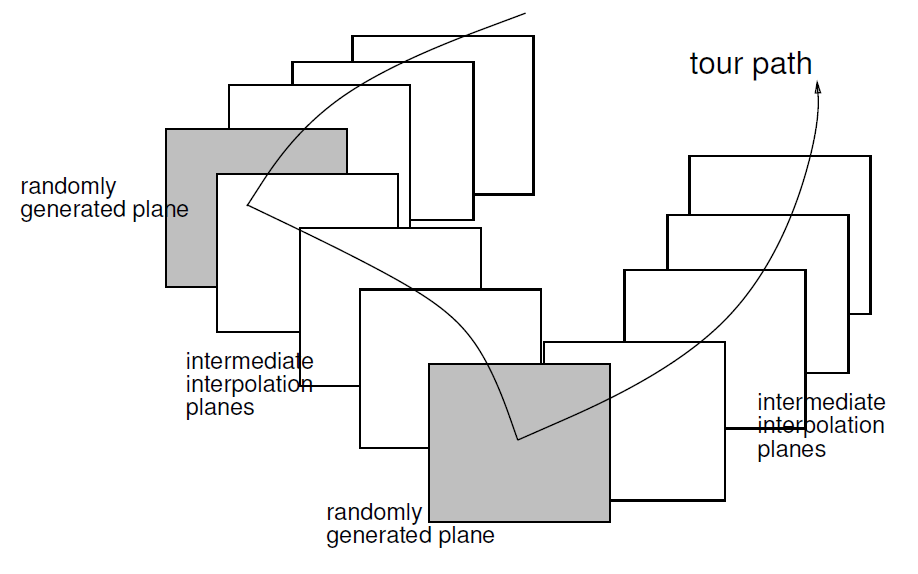
\includegraphics[width=0.8\linewidth]{figures/buja05fig} 

}

\caption{Simlified illustration of a grand tour target and interim frames  (Buja et al. 2005)}\label{fig:grandFrames}
\end{figure}

The \emph{guided} tour (Cook, Buja, and Cabrera 1993) makes use of
projection pursuit (Kruskal 1969; Kruskal 1972) to identify a path. Here
a selected index function is selected. Starting from the initial basis
several nearby bases are checked to see if they perform better on the
index function. If so, this new basis is moved and nearby bases are
checked again in an iterative process. If the closest bases do not
perform better, bases slightly further away are checked as in simulated
annealing (Kirkpatrick, Gelatt, and Vecchi 1983). If no better basis is
identified within the selected stopping criterium, the algorithm stops.

The discrete methods above identity bases that highlight some feature.
The above tours can help understand the structure leading to and from
certain projections. To explore higher dimensional spaces visually, we
need \emph{human-in-the-loop} (Karwowski 2006) tools. We need to be able
to choose and direct the change to a basis. (Cook and Buja 1997)
introduces the idea of the \emph{manual} tour. In a manual tour, an
individual variable is selected as the manipulation variable. Its
contribution to the basis is then controlled. The contributions of the
remaining variables also change as they perform an
orthogonally-constrained rotation. Figure \ref{fig:manipSpace} This
allows for the exploration of a given projection as defined by the user.

\begin{figure}

{\centering 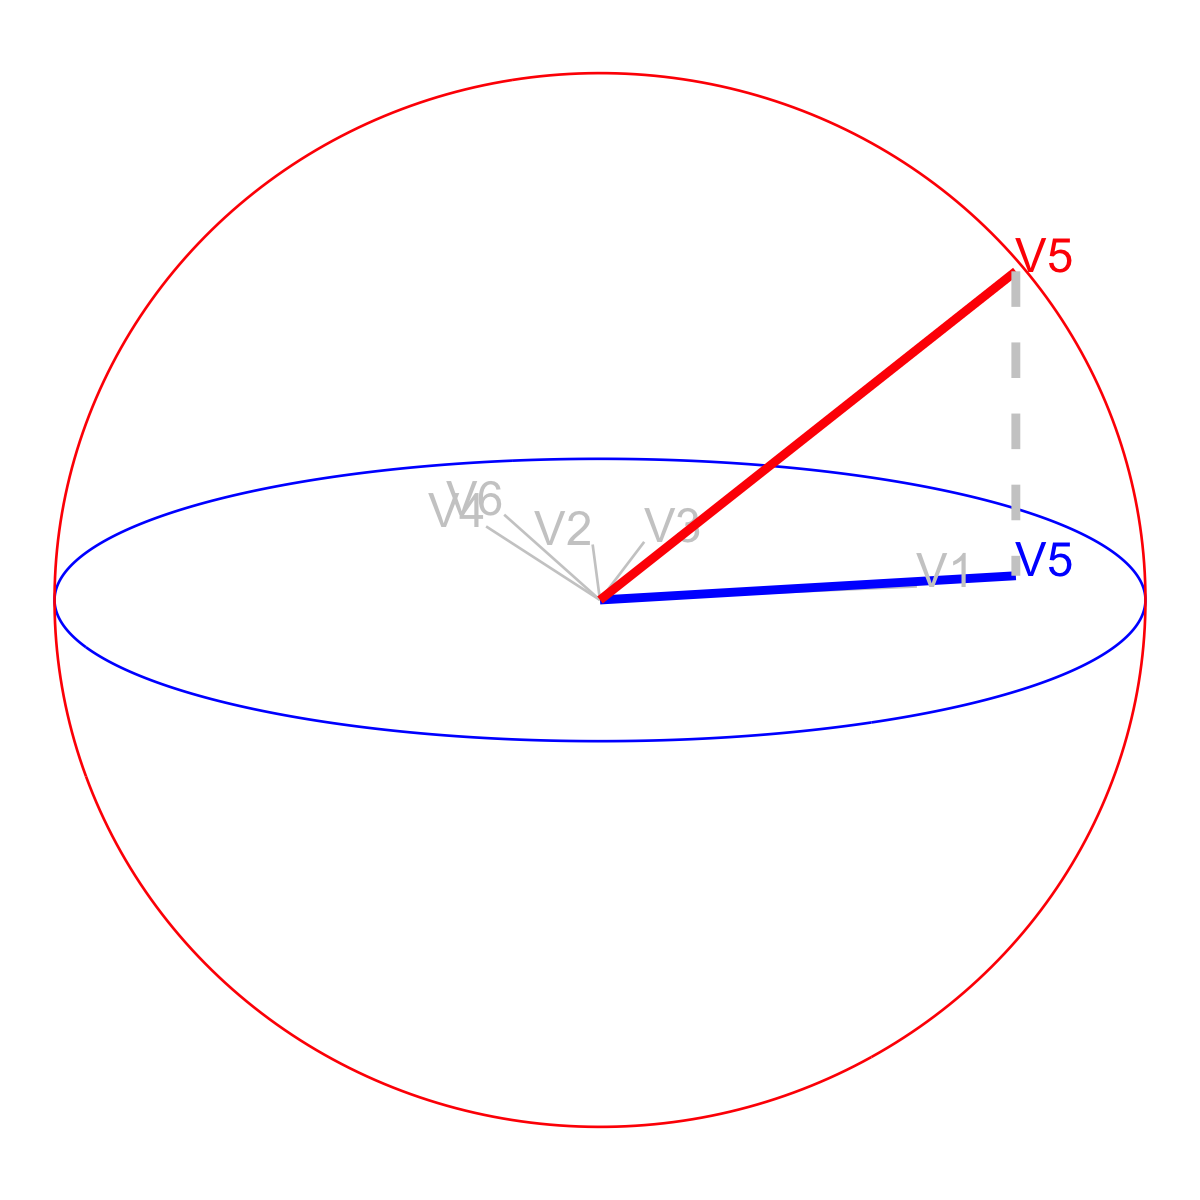
\includegraphics[width=0.5\linewidth]{figures/manip_space} 

}

\caption{Manipulation space of a manual tour. Variable 5 is being manipulated as though the red segment is rotated about the origin changing the contribution of all variables on the basis axes on the blue projection plane.}\label{fig:manipSpace}
\end{figure}

\subsection{Research objectives}\label{research-objectives}

Data and models are typically high-dimensional, with many variables and
parameters. Developing new methods to visualize high dimensions has been
a pursuit of statisticians, computer scientists and visualization
researchers for decades. As technology evolves examining, extending, and
assessing current techniques, in new environments, for new data
challenges, is an important endeavor. The primary objectives of this
Ph.D.~research can then be summarized as the following.

\begin{enumerate}
\def\labelenumi{\arabic{enumi}.}
\item
  \textbf{How can UCS be generalized to work within graphic-specific
  environments for 2D projections?}\\
  Building from the UCS algorithm in Cook and Buja (1997), the algorithm
  should be modified for generalized use with graphic-specific
  environments. This enables fine control to explore the sensitivity of
  structure to the variable contributing to the projection and sets the
  foundation to be used in the remaining objectives.
\item
  \textbf{Does 2D UCS tours provide benefits over alternatives?}\\
  The quality and effectiveness of 2D UCS will be compared with
  alternatives of static, single, linear and non-linear projection
  techniques. They will be quantified by the measurement of structure,
  variation, and clustering across on benchmark datasets.
\item
  \textbf{How can UCS be extended to 3D?}\\
  The addition of a 3rd dimension potentially allows for the improved
  perception of the structure of the data in dynamic UCS. To investigate
  this UCS algorithm needs to be extended to a third dimension. This
  would also allow for novel application multi-parameter function
  projection. This will involve the addition of a new angle and it
  controls the projection space, reference axes, and manipulation space.
  In particular, the manipulation space, now in 4D, will be hard to
  visualize, but it should be able to stand as a mathematical construct
  facilitated through interaction with a point (the projection
  coefficients of the selected manipulation variable) on the now 3D
  reference axes volume.
\end{enumerate}

\subsection{Methodology}\label{methodology}

This research is interdisciplinary; touring was developed by
statisticians to explore physics data. Modern advances in hardware from
information technology allow for 3D rending in higher quality and
immersion than previously possible. Looping back to the original use
care, applications in high energy physics identified (Cook, Laa, and
Valencia 2018).

The research corresponding with RO \#1 entails \emph{algorithm design}
following and further clarifying the work done in Cook and Buja (1997).
In the application of the manual tour, we clarified the creation of the
rotation matrix. The key to the matrix is to specify the 2 axes of
rotation for the manipulation space and apply Rodegeze's formula. In the
application, attention was given to both pre-compiled tour and
human-in-the-loop UCS. We provide an open-source version of the manual
tour in the R package, \texttt{spinifex}, which has since been published
on CRAN. This forms the foundation for future work in the remaining
objectives.

The second objective is addressed with a benchmark dataset
\emph{performance comparison} between dynamic linear projections and
alternatives (static linear and static non-linear projections such as
principal component analysis, multidimensional scaling, and
t-distributed neighbor embeddings, described in more detail in chapter
\ref{ch:future_work}). Benchmark datasets will be compared across
techniques, measurements will include variation explained, transparency
to the original variable space, clustering identification, and outlier
identification.

The research resulting from RO \#2 is a controlled \emph{experimental
study} to explore the efficacy of interactive UCS compared with the
benchmarks factors of PCA and the grand tour. This is designed as a
within-participant study where each participant performs all factors.
the study is balanced by assigning participants into one of 3 groups
where the factor order is controlled by a Latin square while simulation
order remains the same.

The research for RO \#3 involves \textbf{algorithm design}, where the
work in RO \#1 will be extended to display with the use of a third
spatial dimension. This will also be used to develop visualizations of
projected multi-dimension function surfaces. This forms the calculation
base for the work. Several difficulties may arise when bringing dynamic
projection into 3D spaces, especially when exploring 3D surfaces
(discussed in more detail in chapter \ref{ch:future_work}).

\section{Progress since confirmation}\label{progress-since-confirmation}

During the candidature confirmation review (27 March 2019) we discussed
exploratory data analysis, visualization of high dimensional spaces,
covered the literature for tours and 3D rendering for information
perception. We concluded with a process for a manual tour that allows
for user-controlled steering. The appending the document was a mostly
complete R package and respective paper providing an open-source
application as well as clarifying the rotation matrix that was outlined
in Cook and Buja (1997).

\subsection{Publication}\label{publication}

The paper has since been accepted in the R Journal and it currently
undergoing editorial review. This will be published in the first issue
of 2020 and available at
\href{https://journal.r-project.org/}{journal.r-project.org}.

\subsection{Software}\label{software}

The R package, \texttt{spinifex\ (v0.1.0)}, has been approved and hosted
for public use on the Comprehensive R Archival Network, CRAN
(cran.r-project.org/web/packages/spinifex/)(\url{https://cran.r-project.org/web/packages/spinifex/index.html}).

New functionality has been added to the development branch, specifically
around the interactive use. A user application is developed with
\texttt{shiny}(Chang et al. 2018). It allows users to explore their data
without the need for coding familiarity. It features interactive or
precompiled manual touring. It also contains a gallery for flagging
bases which can then further be reviewed or saved as .gif and .png
files.

\subsection{Experimental study}\label{experimental-study}

The prominent appeal of the manual tour is that it allows users to
control the contributions of individual variables. In theory, this
should enable the finer exploration of features of interest. The
hypothesis we will study is \emph{Does the finer control afforded}
\emph{by the manual tour improve the ability of the analyst to
understand the} \emph{importance of variables contributing to the
structure?}

\section{Proposed thesis structure}\label{proposed-thesis-structure}

\subsection{Structure}\label{structure}

\textbf{Thesis}

\begin{itemize}
\tightlist
\item
  Introduction -- 60\%
\item
  Literature review -- 80\%
\item
  Manual tour and user-controlled steering -- 90\%
\item
  Experimental study -- 40\%
\item
  The extension of the manual tour to 3D -- 0\%
\item
  Conclusion and future plans -- 0\%
\end{itemize}

\begin{figure}

{\centering 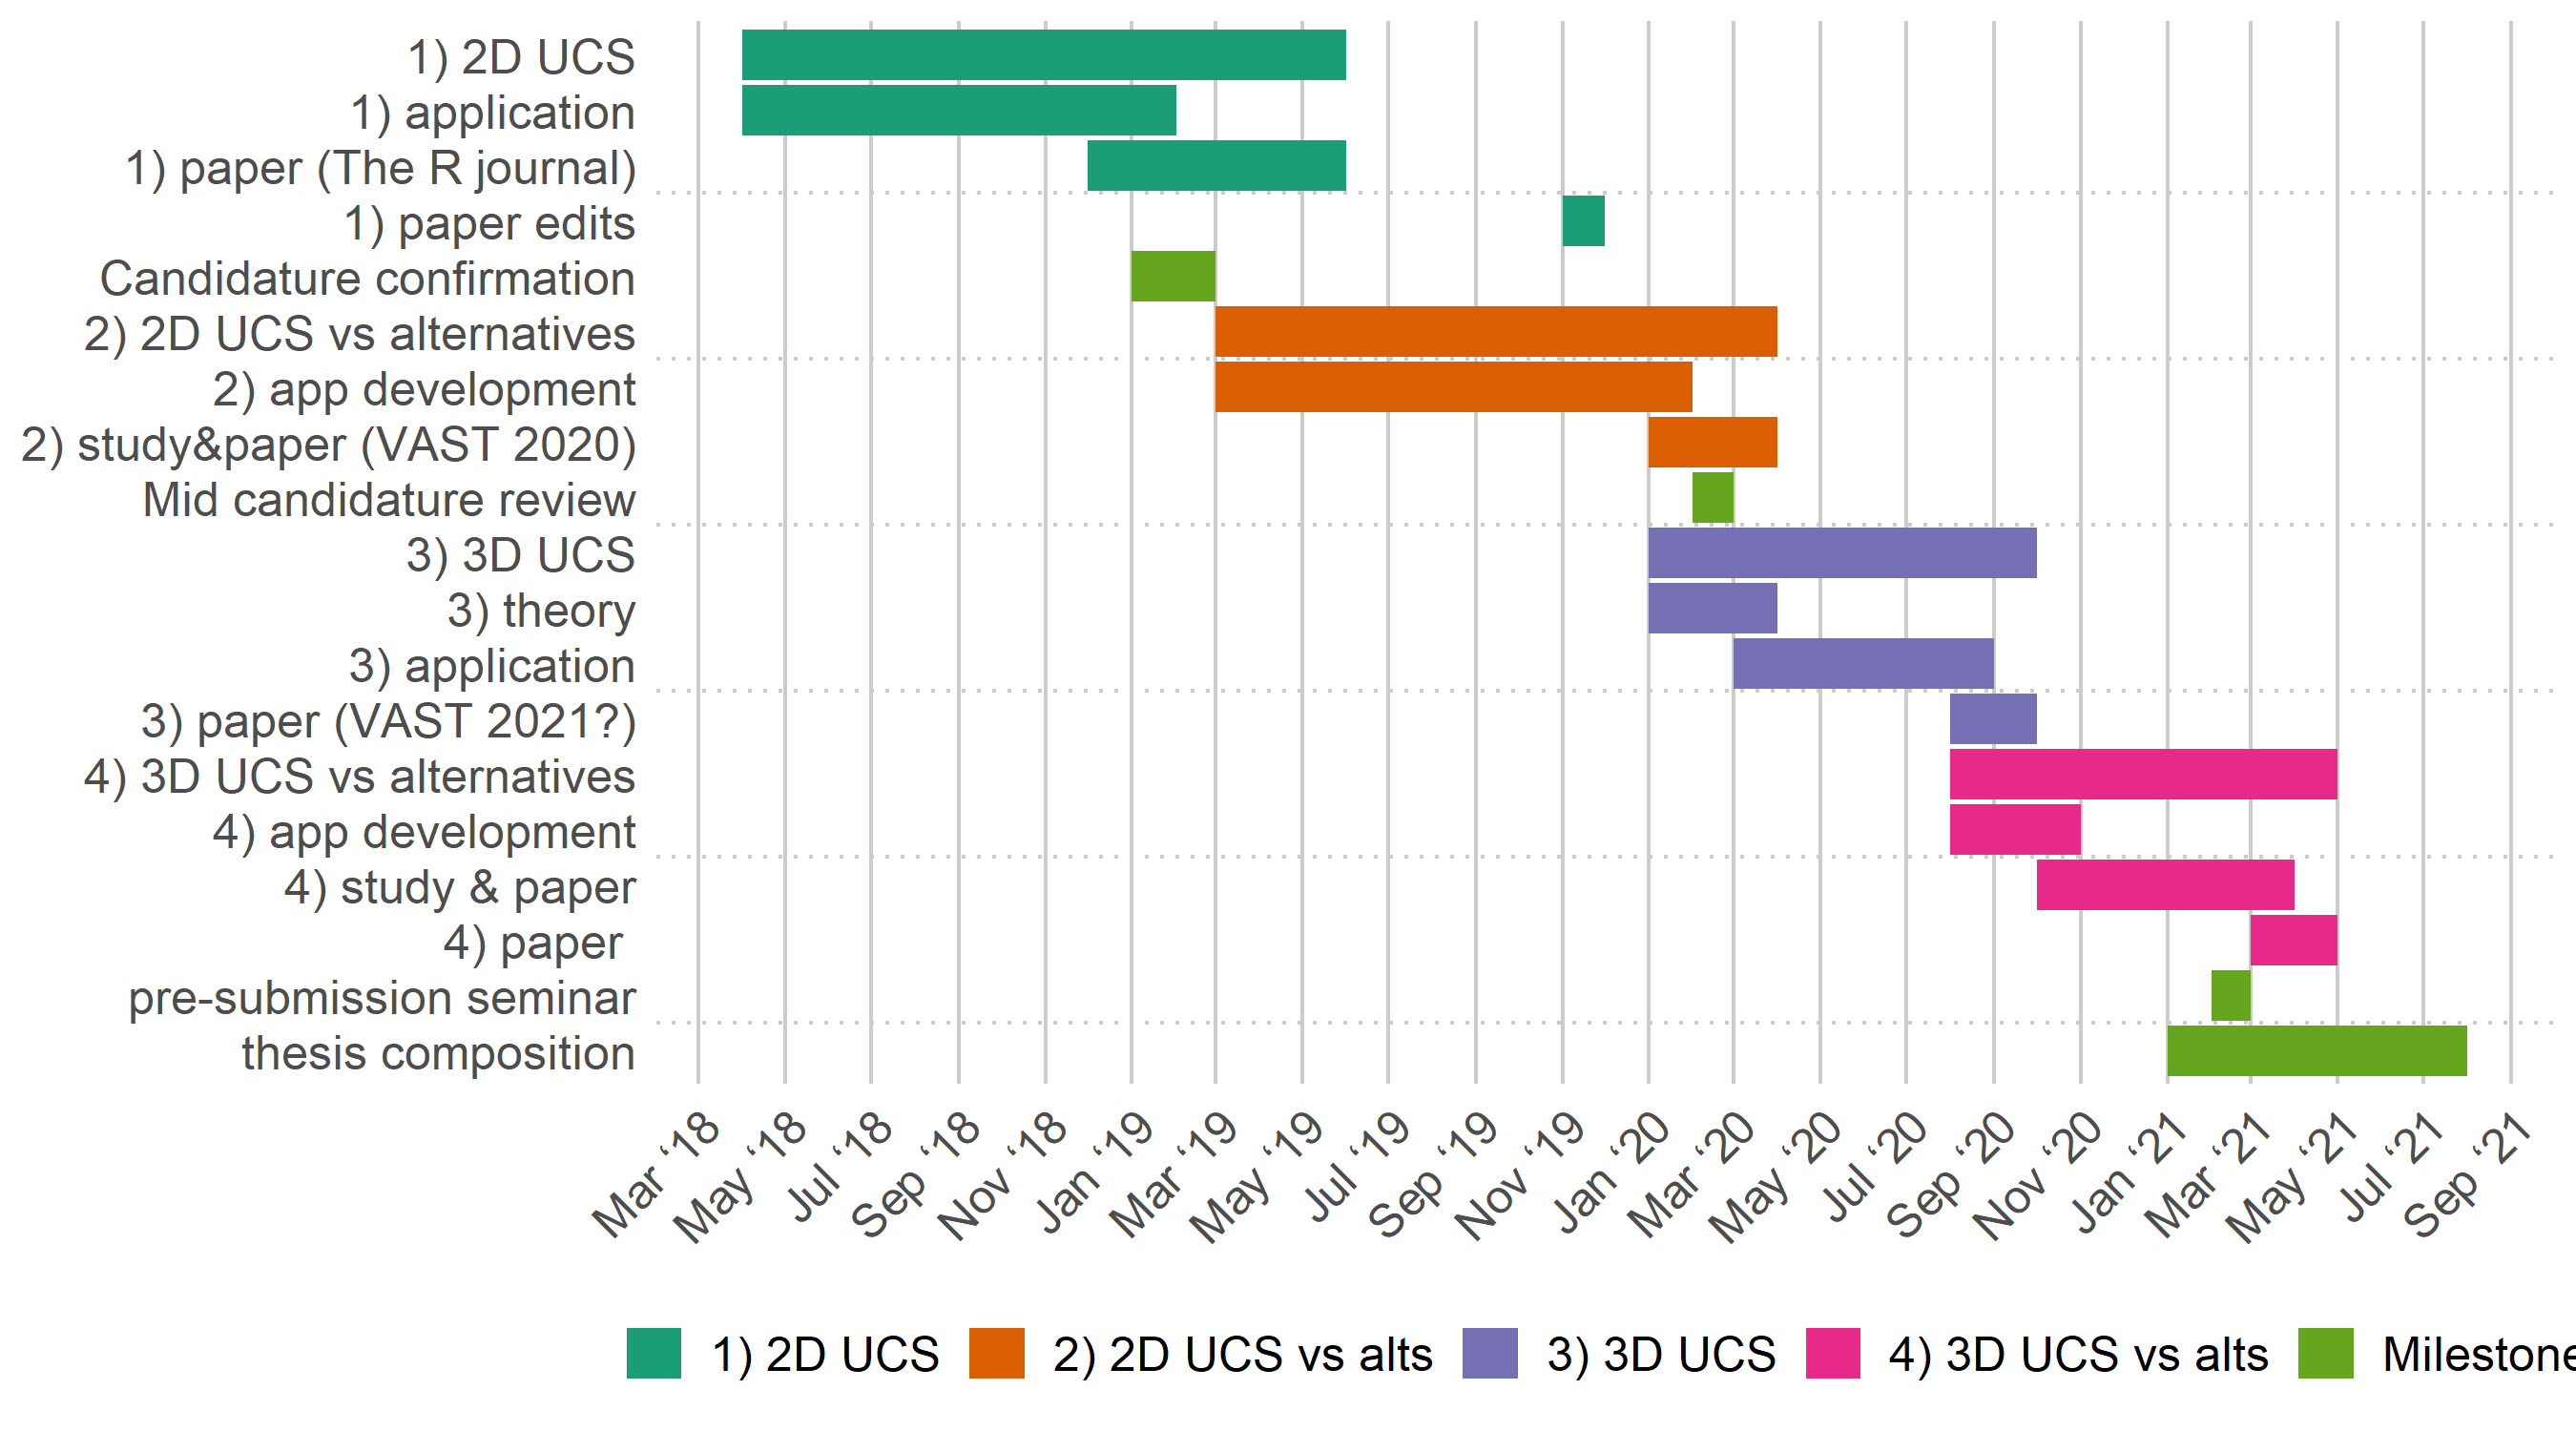
\includegraphics[width=1\linewidth]{figures/phd_timeline} 

}

\caption{Proposed research timeline.}\label{fig:timeline}
\end{figure}

\subsection{Program requirements}\label{program-requirements}

\begin{itemize}
\tightlist
\item
  WES Academic record

  \begin{itemize}
  \tightlist
  \item
    FIT5144: 2019 S1+2, \textbf{In progress}, extended to the
    pre-submission seminar with the unit coordinator for the usual 2
    opportunities to complete.

    \begin{itemize}
    \tightlist
    \item
      Hours: 147\textgreater{}120 hours \textbf{Tracked}, followng
      required (12 hr total)
    \item
      \emph{Needed:} CYR 2 (A \& B) -- 2x 3hr
    \item
      \emph{Needed:} Faculty of IT Workshop 1 and 3 on Ethical Research
      and Publishing -- 2x 3hr
    \end{itemize}
  \item
    FIT5113: 2018 S2, \textbf{Exemption} 
  \item
    FIT6021: 2018 S2, \textbf{Completed} with distinction
  \end{itemize}
\item
  myDevelopment - IT: Monash Doctoral Program - Compulsory Module

  \begin{itemize}
  \tightlist
  \item
    Monash graduate research student induction: \textbf{Completed} 
  \item
    Research Integrity - Choose the Option most relevant:
    \textbf{Completed} 
  \item
    Faculty Induction: \textbf{Completed} 
  \end{itemize}
\end{itemize}

\section{Potential issues for panel to
consider}\label{potential-issues-for-panel-to-consider}

\subsection{Funding for human
subjects}\label{funding-for-human-subjects}

\begin{itemize}
\tightlist
\item
  Beverage voucher: \$5 x 24 people (est) = \$120
\end{itemize}

\subsection{Support for conference
travel}\label{support-for-conference-travel}

\textbf{Conferences:}\\[2\baselineskip]CHI 2021: May 8-13, 2021
Yokohama, Japan\\
submission: Thursday Sep. 10, 2020 (+ 1wk for full)\\
\url{https://chi2021.acm.org/}\\[2\baselineskip]IEEE VIS - SciVis 2020:
25-30 October 2020 Salt Lake City, Utah, USA\\
submission: Saturday, March 21, 2020 (+ 10 days for full) SciVis -
Empirical Study\\
\url{http://ieeevis.org/year/2020/info/call-participation/scivis-paper-types}

\section{Acknowledgements}\label{sec:acknowledgements}

This report was created in \texttt{R} (R Core Team 2019), using
\texttt{bookdown} (Xie 2016) and \texttt{rmarkdown} (Xie, Allaire, and
Grolemund 2018).

For version control, transparency, and reproducibility, the source files
are made available found at
\href{https://github.com/nspyrison/mid_canidature}{github.com/nspyrison/mid\_canidature}.

\section*{References}\label{references}
\addcontentsline{toc}{section}{References}

\hypertarget{refs}{}
\hypertarget{ref-anscombe_graphs_1973}{}
Anscombe, F. J. 1973. ``Graphs in Statistical Analysis.'' \emph{The
American Statistician} 27 (1): 17--21.
doi:\href{https://doi.org/10.2307/2682899}{10.2307/2682899}.

\hypertarget{ref-asimov_grand_1985}{}
Asimov, Daniel. 1985. ``The Grand Tour: A Tool for Viewing
Multidimensional Data.'' \emph{SIAM Journal on Scientific and
Statistical Computing} 6 (1): 128--43.
doi:\href{https://doi.org/https://doi.org/10.1137/0906011}{https://doi.org/10.1137/0906011}.

\hypertarget{ref-buja_grand_1986}{}
Buja, Andreas, and Daniel Asimov. 1986. ``Grand Tour Methods: An
Outline.'' In \emph{Proceedings of the Seventeenth Symposium on the
Interface of Computer Sciences and Statistics on Computer Science and
Statistics}, 63--67. New York, NY, USA: Elsevier North-Holland, Inc.
\url{http://dl.acm.org/citation.cfm?id=26036.26046}.

\hypertarget{ref-cattell_scree_1966}{}
Cattell, Raymond B. 1966. ``The Scree Test for the Number of Factors.''
\emph{Multivariate Behavioral Research} 1 (2): 245--76.

\hypertarget{ref-chambers_graphical_1983}{}
Chambers, J.M., W.S. Cleveland, B. Kleiner, and P.A. Tukey. 1983.
``Graphical Methods for Data Analysis.''

\hypertarget{ref-chang_shiny:_2018}{}
Chang, Winston, Joe Cheng, J. J. Allaire, Yihui Xie, and Jonathan
McPherson. 2018. \emph{Shiny: Web Application Framework for R}.
\url{https://CRAN.R-project.org/package=shiny}.

\hypertarget{ref-cook_manual_1997}{}
Cook, Dianne, and Andreas Buja. 1997. ``Manual Controls for
High-Dimensional Data Projections.'' \emph{Journal of Computational and
Graphical Statistics} 6 (4): 464--80.
doi:\href{https://doi.org/10.2307/1390747}{10.2307/1390747}.

\hypertarget{ref-cook_projection_1993}{}
Cook, Dianne, Andreas Buja, and Javier Cabrera. 1993. ``Projection
Pursuit Indexes Based on Orthonormal Function Expansions.''
\emph{Journal of Computational and Graphical Statistics} 2 (3): 225--50.
doi:\href{https://doi.org/10.1080/10618600.1993.10474610}{10.1080/10618600.1993.10474610}.

\hypertarget{ref-cook_dynamical_2018}{}
Cook, Dianne, Ursula Laa, and German Valencia. 2018. ``Dynamical
Projections for the Visualization of PDFSense Data.'' \emph{Eur. Phys.
J. C} 78 (9): 742.
doi:\href{https://doi.org/10.1140/epjc/s10052-018-6205-2}{10.1140/epjc/s10052-018-6205-2}.

\hypertarget{ref-karwowski_international_2006}{}
Karwowski, Waldemar. 2006. \emph{International Encyclopedia of
Ergonomics and Human Factors, -3 Volume Set}. CRC Press.

\hypertarget{ref-kirkpatrick_optimization_1983}{}
Kirkpatrick, Scott, C. Daniel Gelatt, and Mario P. Vecchi. 1983.
``Optimization by Simulated Annealing.'' \emph{Science} 220 (4598):
671--80.
doi:\href{https://doi.org/10.1126/science.220.4598.671}{10.1126/science.220.4598.671}.

\hypertarget{ref-kohonen_self-organizing_1990}{}
Kohonen, Teuvo. 1990. ``The Self-Organizing Map.'' \emph{Proceedings of
the IEEE} 78 (9): 1464--80.

\hypertarget{ref-kruskal_toward_1969}{}
Kruskal, Joseph B. 1969. ``Toward a Practical Method Which Helps Uncover
the Structure of a Set of Multivariate Observations by Finding the
Linear Transformation Which Optimizes a New `Index of Condensation'.''
In \emph{Statistical Computation}, edited by Roy C. Milton and John A.
Nelder, 427--40. Academic Press.
doi:\href{https://doi.org/10.1016/B978-0-12-498150-8.50024-0}{10.1016/B978-0-12-498150-8.50024-0}.

\hypertarget{ref-kruskal_linear_1972}{}
---------. 1972. ``Linear Transformation of Multivariate Data to Reveal
Clustering.'' \emph{Multidimensional Scaling: Theory and Applications in
the Behavioral Sciences} 1: 181--91.

\hypertarget{ref-maaten_visualizing_2008}{}
Maaten, Laurens van der, and Geoffrey Hinton. 2008. ``Visualizing Data
Using T-SNE.'' \emph{Journal of Machine Learning Research} 9 (Nov):
2579--2605.

\hypertarget{ref-matejka_same_2017}{}
Matejka, Justin, and George Fitzmaurice. 2017. ``Same Stats, Different
Graphs: Generating Datasets with Varied Appearance and Identical
Statistics Through Simulated Annealing.'' In \emph{Proceedings of the
2017 CHI Conference on Human Factors in Computing Systems - CHI '17},
1290--4. Denver, Colorado, USA: ACM Press.
doi:\href{https://doi.org/10.1145/3025453.3025912}{10.1145/3025453.3025912}.

\hypertarget{ref-pearson_liii._1901}{}
Pearson, Karl. 1901. ``LIII. on Lines and Planes of Closest Fit to
Systems of Points in Space.'' \emph{The London, Edinburgh, and Dublin
Philosophical Magazine and Journal of Science} 2 (11): 559--72.

\hypertarget{ref-r_core_team_r:_2019}{}
R Core Team. 2019. \emph{R: A Language and Environment for Statistical
Computing}. Vienna, Austria: R Foundation for Statistical Computing.
\url{https://www.R-project.org/}.

\hypertarget{ref-tukey_exploratory_1977}{}
Tukey, John W. 1977. \emph{Exploratory Data Analysis}. Vol. 32. Pearson.

\hypertarget{ref-wickham_tourr:_2011}{}
Wickham, Hadley, Dianne Cook, Heike Hofmann, and Andreas Buja. 2011.
``Tourr: An R Package for Exploring Multivariate Data with
Projections.'' \emph{Journal of Statistical Software} 40 (2).
doi:\href{https://doi.org/10.18637/jss.v040.i02}{10.18637/jss.v040.i02}.

\hypertarget{ref-xie_bookdown:_2016}{}
Xie, Yihui. 2016. \emph{Bookdown: Authoring Books and Technical
Documents with R Markdown}. Boca Raton, Florida: Chapman; Hall/CRC.
\url{https://github.com/rstudio/bookdown}.

\hypertarget{ref-xie_r_2018}{}
Xie, Yihui, J. J. Allaire, and Garrett Grolemund. 2018. \emph{R
Markdown: The Definitive Guide}. Boca Raton, Florida: Chapman; Hall/CRC.
\url{https://bookdown.org/yihui/rmarkdown}.

\end{document}
